\chapter{Crystal growth review and measurements}\label{chap_growth}
\graphicspath{{./growth/graphs/}}

In the previous chapter we discussed the thermodynamics of polymer crystallization, while this process is in fact controlled by kinetics more than thermodynamics due to the nature of polymers. Kinetic theories typically analyze a process from two aspects: "driving force" and "free energy barrier" \cite{Zhang2016a}. "Driving force" in the case of polymer crystallization refers to the free energy difference between the crystalline state and the amorphous state, and "free energy barrier" includes all kinds of factors that are against the crystallization process, such as entanglement of chains, defects in the system, etc. These two factors compete with each other, and the system reaches the most stable state by balancing them.

\section{Crystallization with spherulites}

When a polymer crystal is grown from a melt, superstructures called spherulites are normally formed. These structures are composed of stacked lamellae that have grown from a common centre, as shown in Figure \ref{fig:spherulite}. Spherulites are normally formed when there is no thermal gradient present, because in the presence of thermal gradient with a certain direction, crystal growth would follow the gradient instead of growing radially \cite{Carraher2003}. In spherulites, polymer chains are aligned perpendicular to the radius of the spherulite. During crystallization, the spherulites grow until they contact each other, and their sizes range from microns to millimeters \cite{Vasile2000}, which can be easily observed under an optical microscope. Among the crystalline stacks are amorphous regions, together forming a semicrystalline structure.

\begin{figure}[H]
\center
\includegraphics[width=0.4\linewidth]{spherulite}
\caption[A polymer spherulite with folded-chain lamellae.]{A polymer spherulite with folded-chain lamellae. Figure source: "The Morphology of Crystalline Synthetic Polymers" by F. Khoury and E. Passaglia, \textit{Treatise Solid State Chem.}, pages 335–496, 1976 \cite{Khoury1976}.}
\label{fig:spherulite}
\end{figure}

The growth of a spherulite is controlled by many factors including the number of nucleation sites, polymer structure, crystallization temperature, cooling rate, etc. For example, if the crystallization temperature is low enough or there are a large number of present nuclei, many spherulites would be created and grow into relatively small sizes; while if the supercooling is small, and fewer nuclei are present, fewer spherulites would form, but they would be larger in size \cite{LindaSawyerDavidT.Grubb2008}. Spherulites are optically anisotropic because of the alignment of the linear polymer chains. When they are viewed under an optical microscope, with crossed polarizers on, certain patterns such as the "Maltese cross" consisting of eight alternating bright and dark fan-shaped areas (Figure \ref{fig:Maltese cross}) are often observed, resulting from the birefringence of the lamellae \cite{Bower2002}.

\begin{figure}[H]
\center
\includegraphics[width=0.3\linewidth]{Maltese}
\caption{Optical microscope image (with crossed polarizers on) of fraction with $\bar{N} = 12.4$ at 260.65 K.}
\label{fig:Maltese cross}
\end{figure}

\subsection{Nucleation} \label{nucleation}

Crystallization can be divided into two stages: nucleation and crystal growth. Nucleation is the primary step in the crystallization of a polymer. As temperature decreases, a polymer normally does not crystallize immediately when it reaches the melting temperature, but rather needs a considerable supercooling before crystallization. The reason is that crystallization starts with nucleation, and if the polymer sample has little or no nuclei present, the temperature is able to kept decreasing until the sample grows a nucleus from itself, which is called primary nucleation. The driving force of this process is the local density fluctuation, and it is able to occur at temperatures below the melting temperature and above the glass transition temperature.

Apart from primary nucleation, there are also secondary and tertiary nucleation. If we consider the formation of a cubic nucleus, primary nucleation requires 6 new faces to be formed, while secondary nucleation requires 4 new faces (on the surface of present nuclei), and tertiary nucleation requires only 2 new faces (at the edge of present nuclei) \cite{Chai2016}.

Primary nucleation is further classified into homogeneous nucleation and heterogeneous nucleation. Homogeneous nucleation refers to a nucleation process that is purely induced by thermal fluctuations and does not involve the influence of any solids, including present crystal, container walls, or foreign particles present in the crystallizing sample. Heterogeneous nucleation, however, refers to a primary nucleation with the help of impurity particles, either uncontrolled or deliberately introduced into the sample \cite{Strobl2007a}. Homogeneous nucleation will be mainly focused on here, but heterogeneous nucleation is much more common in real cases. Foreign particles help greatly reduce the free energy barrier of the phase transition from liquid to crystal, and lead to a smaller supercooling.

In a homogeneous nucleation process, thermal fluctuations result in the formation of embryos (small aggregates with enhanced inner order), and the size of the embryos determines if they could survive through the energy barrier and grow into a larger crystal. If the embryo is not big enough, there would only be a small free energy loss caused by crystallization, compared to the free energy barrier in creating their surfaces. In this case, the embryo can not survive and would have to melt. Assuming the embryos are spherical, the classical nucleation theory can be applied to derive the critical size of an embryo \cite{Chai2016}.

The total free energy of an embryo is:

\begin{equation}
\label{eqn_delta G of embryo}
\Delta G = -\dfrac{4}{3} \pi r^{3} \Delta g + \sigma_{e} 4 \pi r^{2}
\end{equation}

\noindent
where $r$ is the embryo radius, $\Delta g$ is the free energy per unit mass on melting, and $\sigma_{e}$ is the surface free energy of the embryo.

The plot of $\Delta G$ vs $r$ is shown as Figure \ref{fig:Delta G embryo}. We note that there is a maximum in  $\Delta G$, $\Delta G^{*}$, for a critical $r$ value, $r^{*}$. Below this value, $\Delta G$ increases with $r$, while after surpassing it, $\Delta G$ decreases as $r$ increases. When the thermal fluctuations are strong enough to produce embryos larger than $r^{*}$, the embryos could then grow into crystals. These two critical values can be calculated \cite{Hoffman1997} from Equation \ref{eqn_delta G of embryo} by differentiating $\Delta G$ and equating to zero:

\begin{equation}
\label{eqn_critical radius of embryo}
r^{*} = \dfrac{2\sigma_{e}}{\Delta g}
\end{equation}

\begin{equation}
\label{eqn_critical energy of embryo}
\Delta G^{*} = -\dfrac{16\pi\sigma_{e}^{3}}{3\Delta g^{2}}
\end{equation}

\begin{figure}[H]
\center
\begin{tikzpicture}
\begin{axis}[
    ticks=none,
    axis x line=middle,axis y line=left,
    xlabel = {$r$},
    ylabel = {$\Delta G$},
    ymin=-0.121,ymax=0.2,ylabel style={rotate=-90},
]
\addplot [
    domain=0:1.1, 
    range=-0.121:2
    samples=100, 
    color=blue,
]
{x^2 - x^3};
%\draw [ultra thick, dotted, draw=red] 
%        (axis cs: 0,4/27) -- (axis cs: 2/3,4/27);
%\draw [ultra thick, dotted, draw=red] 
%        (axis cs: 2/3,0) -- (axis cs: 2/3,4/27);
%\node[label={180:{($r^{*}$,$\Delta G^{*}$)}},circle,fill,inner sep=2pt] at (axis cs:2/3,4/27) {};
\addplot[mark=*] coordinates {(2/3,4/27)} node[pin=150:{$r^{*}$,$\Delta G^{*}$}]{} ;
\end{axis}
\end{tikzpicture}
\caption{Total free energy of an embryo $\Delta G$ vs embryo radius $r$, where $r^{*}$ and $\Delta G^{*}$ are the critical radius and the critical free energy, respectively.}
\label{fig:Delta G embryo}
\end{figure}

Intuitively we would expect both $r^{*}$ and $\Delta G^{*}$ to show a negative correlation with the extent of supercooling $\Delta T$, and in fact this can be proved as follows. Assuming that the enthalpy and entropy do not vary significantly near the crystallization temperature, we obtain:

\begin{equation}
\label{eqn_Delta g at Tm}
\Delta g(T_{m}) = \Delta h(T_{m}) - T_{m}\Delta s(T_{m}) = 0
\end{equation}


\begin{equation}
\label{eqn_Delta g at Tc}
\Delta g(T_{c}) = \Delta h(T_{c}) - T_{c}\Delta s(T_{c}) = 0
\end{equation}

Equations \ref{eqn_Delta g at Tm} and \ref{eqn_Delta g at Tc} can be rearranged into Equation \ref{eqn_Delta g Tc}:

\begin{equation}
\label{eqn_Delta g Tc}
\Delta g(T_{c}) = \Delta h(T_{c}) - T_{c} \dfrac{\Delta h(T_{c})}{T_{m}} = \Delta h(T_{c}) \dfrac{T_{m} - T_{c}}{T_{m}} = \Delta h(T_{c}) \dfrac{\Delta T}{T_{m}}
\end{equation}

Within the context of the case of embryo growth, Equation \ref{eqn_Delta g Tc} can be modified to yield Equation \ref{eqn_Delta g of embryo}:

\begin{equation}
\label{eqn_Delta g of embryo}
\Delta g = \Delta h \dfrac{\Delta T}{T_{m}}
\end{equation}

Taking advantage of the relationship between $\Delta g$ and $r^{*}$ in Equation \ref{eqn_critical radius of embryo} and $\Delta G^{*}$ in Equation \ref{eqn_critical energy of embryo}, Equation \ref{eqn_relation for r} and \ref{eqn_relation for G} could be derived:

\begin{equation}
\label{eqn_relation for r}
r^{*} \propto \Delta T^{-1}
\end{equation}

\begin{equation}
\label{eqn_relation for G}
\Delta G^{*} \propto \Delta T^{-2}
\end{equation}

As the crystallization temperature ($T_{c}$) gets lower, corresponding to a larger supercooling $\Delta T$, $r^{*}$ and $\Delta G^{*}$ get smaller, indicating an easier nucleation. In addition, according to the nucleation theory by Turnbull and Fisher \cite{Turnbull1949}, the nucleation rate, $i$, is expressed as:

\begin{equation}
\label{eqn_nucleation rate}
i = i_{0}exp(- \dfrac{\Delta E + \Delta G^{*}}{k T})
\end{equation}

\noindent
where $i_{0}$ is a pre-exponential factor, $\Delta E$ is the nucleation activation energy, and $\Delta G^{*}$ is the critical nucleation energy. The dependency on $\Delta T$ through $\Delta G^{*}$ suggests that the nucleation rate $i$ is higher for a larger supercooling, and thus a faster nucleation. However, we need to be careful that when temperature decreases to near the glass transition temperature, $T_{g}$, chain mobility is highly restricted, which makes it harder for thermal fluctuations to produce nuclei. Therefore, there exists a maximum nucleation rate at a temperature between $T_{g}$ and $T_{c}$.

Nucleation can be described by the nucleation time $\tau _{nuc}$ as well, which is simply the inverse of the nucleation rate, and can be directly measured. The nucleation rate is significantly slower than the crystal growth rate, especially for homogeneous nucleation, which makes it very convenient to measure the rate of these two processes separately. In a study \cite{Massa2004} of homogeneous nucleation in PEO crystallization, the relationship between $\tau _{nuc}$ and the volume of the crystallizable droplets $V$ was shown. Impurity-free discrete PEO droplets are formed through dewetting on a polystyrene film, and cooled under an optical microscope with crossed polarizers to observe the nucleation of each droplet. Figure \ref{fig:tauV} presents their findings.

\begin{figure}[H]
\center
\includegraphics[width=0.5\linewidth]{tauV}
\caption[Volume-normalized time constant, $\tau V$, as a function of temperature.]{Volume-normalized time constant, $\tau V$, as a function of temperature. In the index the averaged dewetted droplet data (solid symbols) are in agreement with data from \cite{Rottele2003} (open symbols), both with linear dependence on $[T_{c}(T_{m}-T_{c})^{2}]^{-1}$ as expected from classical nucleation theory \cite{Strobl2007a}. Figure source: "Homogeneous Crystallization of Poly(Ethylene Oxide) Confined to Droplets: The Dependence of the Crystal Nucleation Rate on Length Scale and Temperature" by Michael V. Massa \textit{et al}, \textit{Phys. Rev. Lett.}, 92(25):255509, jun 2004 \cite{Yeates1984}.}
\label{fig:tauV}
\end{figure}

The observation results show that $\tau _{nuc}$ is inversely proportional to the volume as shown in Equation \ref{eqn_nucleation time}:

\begin{equation}
\label{eqn_nucleation time}
\tau _{nuc} \propto V^{-1}
\end{equation}

At the same crystallization temperature, droplets with different volumes have the same value of the volume-normalized time constant, $\tau V$, and it decreases (meaning increasing rate) exponentially as the supercooling becomes larger. The close agreement between these two sets of data and their huge difference ($\sim 8$ orders of magnitude) in $\tau V$ suggests that the nucleation mechanism is consistent within a huge range of size. The many differences in these two experimental systems indicates that nucleation is dominated by the bulk rather than the surface.

\subsection{Crystal growth}

After nuclei have been formed, the ones with radii larger than $r^{*}$ can grow into larger crystals by adsorbing crystallizable materials. Crystal growth is either diffusion-controlled or interface-controlled.

Crystals growing from dilute solutions are typically diffusion-controlled, since in such cases the growth rate depends on the diffusion rate of the crystallizable material onto the surfaces of nuclei. According to Fick's diffusion law \cite{Fick1855,FickZiirich1995}, the relationship between the radius of a crystal $r$ and time $t$ has been found to be well-represented by Equation \ref{eqn_diffusion crystal radius} \cite{Ouyang1998,Ouyang1999,HaoOuyang2004,Naga2013}:

\begin{equation}
\label{eqn_diffusion crystal radius}
r \propto t^{\frac{1}{2}}
\end{equation}

When the solution concentration is high, or when the crystal is growing from a melt, the diffusion rate is no longer the limiting factor in its growth, because the nuclei are surrounded by sufficient crystallizable materials. Therefore, it depends more on the attachment of crystallizable material onto existing nuclei. The attachment and the formation of crystal lamellae are well-described by the widely-accepted theory proposed by Lauritzen and Hoffman \cite{Lauritzen,Hoffman,Lauritzen1973}. The theory relates microscopic movements to macroscopic quantities, and has become the most successful theory to describe this process, although it has also been criticized by some researchers saying that it oversimplifies crystal growth by applying a mean field description \cite{Zhang2016a}.

Lauritzen-Hoffman (LH) theory treats crystal growth as a secondary nucleation process, and one of the basic assumptions is that the nucleus is in fact a single stem grown from thermal fluctuations. It then acts as a growth front, and other stems deposit onto its surface and crystallize stem by stem into a lamella, thus creating a new layer through lateral spreading. When the present surface layer is taken up, this spreading process is repeated if another nucleus is formed on top of this layer.

In order to quantify this process, four parameters need to be defined: the surface nucleation rate, $i$; lateral covering rate, $g$; perpendicular growth rate, $G$; the length of surface, $L$. Three regimes are predicted in the model, as shown in Figure \ref{fig:LH theory}.

\begin{figure}[H]
\center
\includegraphics[width=0.3\linewidth]{LHtheory}
\caption[Polymer crystal growth in three regimes in LH theory.]{Polymer crystal growth in three regimes in LH theory. Figure source: "Enthalpic and entropic origins of nucleation barriers during polymer crystallization: the Hoffman–Lauritzen theory and beyond" by Stephen Z.D. Cheng \textit{et al}, \textit{Polymer (Guildf).}, 46(20):8662–8681, sep 2005  \cite{Cheng2005}.}
\label{fig:LH theory}
\end{figure}

In regime \Romannum{1}, $\Delta T$ is low, and according to the nucleation theory \cite{Turnbull1949} mentioned in \ref{nucleation}, the nucleation rate $i$ is low. In the case where $i$ is smaller than $g$, there is enough time for polymer chains to cover the entire surface, since this process is restricted by $i$. The crystal growth rate $G_{\Romannum{1}}$ in this regime is given by Equation \ref{eqn_regime1}:

\begin{equation}
\label{eqn_regime1}
G_{\Romannum{1}} = i b_{0} L
\end{equation}

\noindent
where $b_{0}$ is the thickness of the new layer formed. LH theory describes that after nucleation (rate-controlling process) takes place, new stems cover the surface by fast lateral growth, and form a new growth front awaiting the next round of nucleation.

As $T_{c}$ decreases, $\Delta T$ increases, and the crystal growth reaches regime \Romannum{2}, where $i$ is now comparable to $g$, and multiple nuclei could be formed at the same time. The growth rate is then dependent on both $i$ and $g$:

\begin{equation}
\label{eqn_regime2}
G_{\Romannum{2}} = (i b_{0} g)^{\frac{1}{2}}
\end{equation}

In this regime, the surface is less smooth than that in regime \Romannum{1}, since multiple nuclei are present when new stems crystallize onto the surface.

At even lower $T_{c}$, $\Delta T$ keeps decreasing, and the crystal growth reaches regime \Romannum{3}, where $i$ becomes larger than $g$, and the separation between two neighbouring nuclei decreases to be comparable to the stem width, so the chains could quickly cover the surface. In this case, the crystal growth rate is again dominated by $i$:

\begin{equation}
\label{eqn_regime3}
G_{\Romannum{3}} = i b_{0} L'
\end{equation}

\noindent
where $L'$ is the separation between neighbouring nuclei, which is normally about 1-3 stem widths \cite{Hoffman1983}. Neighbouring nuclei are so close to each other that the lateral growth rate, $g$, is not significant in this regime. The crystal surface is even rougher than that in regime $\Romannum{2}$.

As previously mentioned, LH theory treats crystal growth as a secondary nucleation process, and thus the crystal growth rate should have a similar dependence on temperature as the nucleation rate does. Figure \ref{fig:growth rate vs T} shows the dependence of the growth rate on temperature for spherulites of isotactic-polystyrene, poly($\epsilon$-caprolactam) (nylon) and poly(tetramethyl-$p$-silphenylene siloxane) (TMPS). The maximum growth rate occurs at a temperature between the glass transition temperature $T_{g}$ and the melting temperature $T_{m}$, as expected from the nucleation process.

\begin{figure}[H]
\center
\includegraphics[width=0.6\linewidth]{GvsT}
\caption[Temperature dependence of the radial growth rate $u$ of spherulites of iPS, nylon and TMPS.]{Temperature dependence of the radial growth rate $u$ of spherulites of iPS, nylon and TMPS. Figure source: "Nucleation and Crystallization" by Gaylon S. Ross \textit{et al}, \textit{Methods Exp. Phys}, 16:339–397, jan 1980 \cite{Ross1980}.}
\label{fig:growth rate vs T}
\end{figure}


%Crystallinity (437A deleted)

%Crystallinity is defined as the volume fraction of crystalline part in a sample. As polymer liquid turns into crystal, its crystallinity can be modeled using Avrami equation (Avrami, 1939). In deriving this equation, some assumptions are made: nucleation is random and homogeneous across the sample; the growth rate is constant and is the same in all directions, which means the nuclei are spherical. (Jena & Chaturvedi, 1992) Define I0 as the nucleation rate per unit volume, and G as the growth rate. Since crystallization can only take place in liquid, the volume of crystallized material needs to be excluded. However, to simplify the calculation, first take the entire sample as liquid. From time τ to τ+dτ, where 0<τ<t, the number of nuclei formed is
%N=VI_0 dτ.
%Since the radius of a nucleus r is G(t-τ), the crystallized volume is given by
%dV_c^'=4π/3 G^3 〖(t-τ)〗^3 VI_0 dτ.
%Integrating from 0 to t leads to
%V_c^'=π/3 VI_0 G^3 t^4.
%As a matter of fact, the volume of previously crystallized material needs to be excluded. The real volume is
%dV_c=1-V_c/V dV_c'.
%Therefore 
%dV_c^'=1/(1-V_c/V) dV_c.
%By integration, 
%ln⁡(1-Y)=-(V_c^')/V=-π/3 I_0 G^3 t^4,
%where Y=V_c/V is the relative crystallinity. Thus 
%1-Y=exp⁡(-π/3 I_0 G^3 t^4).
%The general form of Avrami equation is given by 
%Y=1-exp⁡(-Kt^n).
%In this special case, K=π/3 I_0 G^3, and n=4.

\section{Review of PEO oligomers crystal growth rate}

The crystal growth rate of PEO oligomers, the polymer investigated in this thesis, has been investigated by many researchers. One of the earliest and most famous studies was done by Kovacs \textit{et al} \cite{Kovacs1975}. Figure \ref{fig:Kovacs} and Figure \ref{fig:Kovacs2} show the growth rates vs temperature and molecular weight. 

\begin{figure}[H]
\center
\includegraphics[width=0.55\linewidth]{Kovacs}
\caption[PEO crystal growth rate with respect to temperature and molecular weight.]{PEO crystal growth rate with respect to temperature and molecular weight. Figure source: "Isothermal growth, thickening, and melting of polyethylene oxide) single crystals in the bulk" by A J Kovacs \textit{et al}, \textit{J. Polym. Sci. Polym. Symp.}, 50(1):283-325, 1975 \cite{Kovacs1975}.}
\label{fig:Kovacs}
\end{figure}

\begin{figure}[H]
\center
\includegraphics[width=0.55\linewidth]{Kovacs2}
\caption[Extended-chain PEO crystals growth rate with respect to temperature and molecular weight.]{Extended-chain PEO crystals growth rate with respect to temperature and molecular weight. Figure source: "Isothermal growth, thickening, and melting of polyethylene oxide) single crystals in the bulk. II" by A J Kovacs \textit{et al}, \textit{J. Polym. Sci. Polym. Symp.}, 59(1):31–54, 1975 \cite{Kovacs1977}}.
\label{fig:Kovacs2}
\end{figure}

Two types of growth rates were measured in their study. $G_{R}$ refers to the radial growth rate of spherulites, and $G_{H}$, or $G(010)$, refers to the radial growth rate along the (010) prism faces. For the measurement of $G_{R}$, several low molecular weight PEO samples were sandwiched between cover slips, forming films about \SI{10}{\micro\metre} in thickness, and crystallized at different temperatures. The growth rates of the spherulites were directly measured under an optical microscope with crossed polarizers. For the measurement of $G_{H}$, PEO single crystals were grown from thin molten films with a thickness of about 100 nm, and examined with an electron microscope.

Five low molecular weight samples and one high molecular weight sample were investigated, and from Figure \ref{fig:Kovacs}, $G_{R}$ and $G_{H}$ were found to agree extremely well with each other, showing no significant difference. Both growth rates extended over six orders of magnitudes, and they can be considered to belong to the higher temperature half of Figure \ref{fig:growth rate vs T}, where the growth rate slows down as supercooling decreases. Along the curve of each low molecular weight, there was as least one sharp transition point. These points were believed to be transition temperatures $T(n)$, where the polymer chains in the crystal turned from $n$-times fold to $(n+1)$-times fold. The high molecular weight curve did not display such a transition point.

\section{Optical microscopy experiments}

With our purified products of PEO oligomers, we also did measurements on crystal growth rates under an optical microscope with crossed polarizers. With each sample, we watched crystallization, took a series of pictures at fixed time intervals, as shown in Figure \ref{fig:growth}, and measured the radius of a spherulite in each picture. A graph of crystal size as a function of crystallization time was then generated (Figure \ref{fig:crystal size}), and the growth rate was calculated from the slope of the graph. This process was repeated at different crystallization temperatures, and with fractions having different $\bar{N}$ values.

\begin{figure}[H]
\center
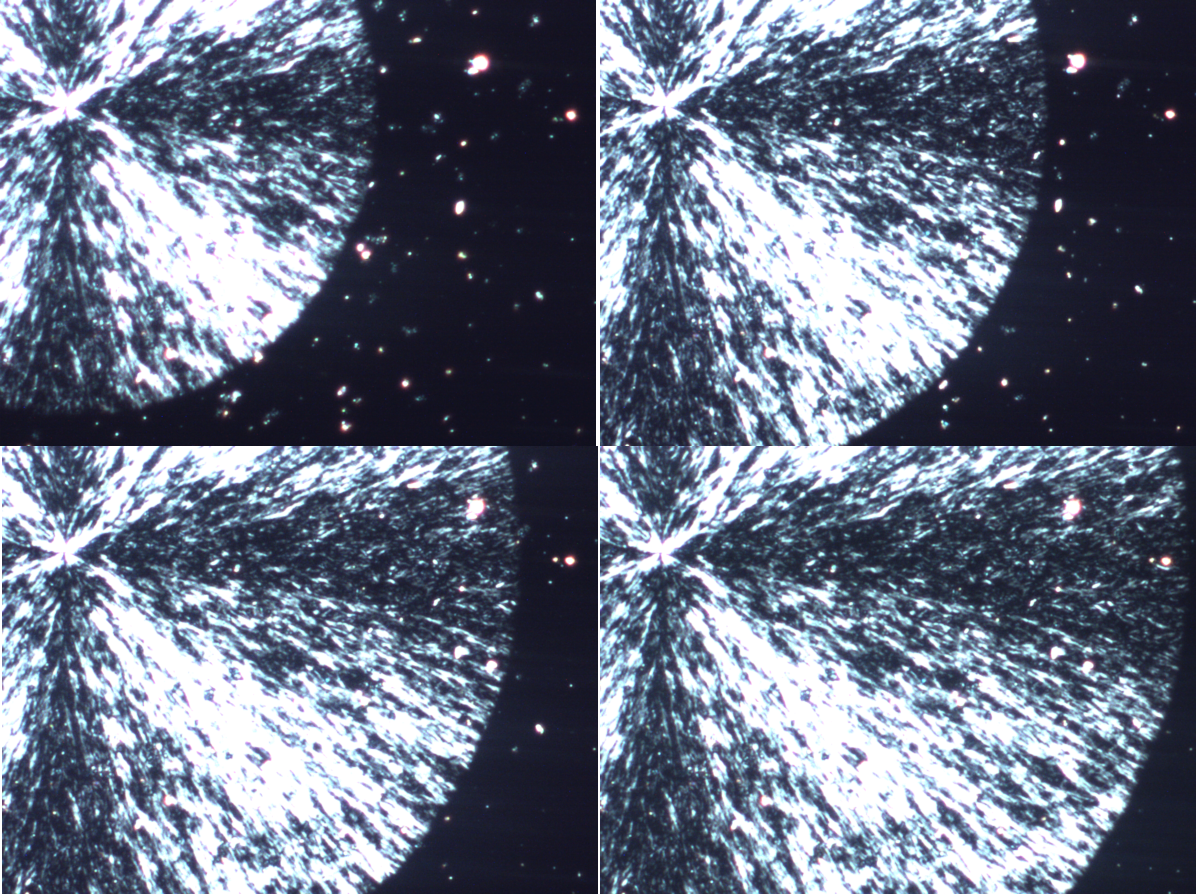
\includegraphics[width=0.5\linewidth]{growth}
\caption{Four sequential images of fraction with $\bar{N} = 12.4$ at 260.65 K, under an optical microscope with crossed polarizers on.}
\label{fig:growth}
\end{figure}

\begin{figure}[H]
	\center
	\includegraphics[width=0.4\linewidth]{crystalsize}
	\caption{Crystal size as a function of crystallization time. $\bar{N} = 12.4$, $T = 260.65 K$.}
	\label{fig:crystal size}
\end{figure}

\section{Crystal growth rate of purified products}

We performed growth rate measurements with four of our fractions, and the results are shown in Figure \ref{fig:logGvsTc}.

\begin{figure}[H]
	\center
	\includegraphics[width=0.5\linewidth]{logGvsTc}
	\caption{Crystal growth rate vs crystallization temperature, with four fractions having different chain lengths. Vertical bars are the melting temperatures of the fractions.}
	\label{fig:logGvsTc}
\end{figure}

At low enough temperatures, the supercooling is large, and fast nucleation, fast crystal growth, and sufficiently bright contrast were obtained. However, at temperatures closer to $T_{m}$, the driving force became small due to small supercooling, which resulted in very difficult nucleation, and the contrast from the crystal was weak so that growth rate could not be measured successfully. Therefore, we have obtained data only for low crystallization temperatures and large growth rates. By looking at the graph itself, we could not find a clear trend, but comparison with Figure \ref{fig:Kovacs} showed good agreement between our data and the low temperature plateau regions in terms of scale in their study. In order to get the full picture of crystal growth of our samples, improvements in experiments are still required to allow us to measure crystallization under small supercoolings, and reach the rapidly decreasing regions as shown in Figure \ref{fig:Kovacs2}.